\documentclass[a4paper,12pt]{scrartcl}
\usepackage{etex}
\usepackage{xltxtra}
\usepackage[babelshorthands]{polyglossia}
\usepackage{graphicx}
\usepackage{color}
\usepackage{hyperref}
\usepackage{amsmath}
\usepackage{unicode-math}
\setmathfont{XITS Math}

\usepackage{moreenum}

\typearea{18}
 
\pagestyle{empty}
\definecolor{linkcol}{rgb}{0.00,0.00,0.50}
\definecolor{urlcol}{rgb}{0.50,0.00,0.00}
\hypersetup{%
  pdftitle={Bildgenerierung, WS 2015/2016},
  pdfauthor={Holger Arndt},
  pdfpagemode=UseThumbs,
  colorlinks=true,
  linkcolor=linkcol,
  urlcolor=urlcol,
}

\setmainlanguage{german}
\defaultfontfeatures{Mapping=tex-text,Scale=MatchLowercase}
\setmainfont[Scale=1]{XITS}
\setsansfont[Scale=0.9]{FreeSans}
\setmonofont[Scale=0.82]{DejaVu Sans Mono}

\renewcommand{\theenumi}{\alph{enumi}}
\renewcommand{\labelenumi}{\theenumi)}

\begin{document}
 
\section*{Lösung zum 3D-Clipping, Theorie}

nacheinander zu testende Fälle:

\begin{enumerate}
\item\label{it:clipz} $-1 ≤ z ≤ z_\text{min}$
\item\label{it:clipx} $z ≤ x ≤ -z$
\item\label{it:clipy} $z ≤ y ≤ -z$
\end{enumerate}

\minisec{Parameterdarstellung der Gerade}

\[ x(t) = x₀ + t (x₁ - x₀) \,\text,\quad y(t) = y₀ + t (y₁ - y₀) \,\text,\quad 
z(t) = z₀ + t (z₁ - z₀) \,\text,\quad 0 ≤ t ≤ 1\]

\begin{itemize}
\item[zu \ref{it:clipz}] \mbox{}
  \begin{enumerate}
  \item $z₀ + t₁ (z₁ - z₀) = -1 ⇔ t₁ = \frac{-1 - z₀}{z₁ - z₀} =
    \frac{z₀ + 1}{z₀ - z₁}$
  \item $z₀ + t₂ (z₁ - z₀) = z_\text{min} ⇔ t₂ = \frac{z_\text{min} - z₀}{z₁ - z₀} =
    \frac{z₀ - z_\text{min}}{z₀ - z₁}$
  \end{enumerate}
\item[zu \ref{it:clipx}] \mbox{}
  \begin{enumerate}
  \item $x₀ + t₁ (x₁ - x₀) = z₀ + t₁ (z₁ - z₀) ⇔ t₁ =
    \frac{z₀ - x₀}{x₁ - x₀ + z₀ - z₁}$
  \item $x₀ + t₂ (x₁ - x₀) = -\left(z₀ + t₂ (z₁ - z₀)\right) ⇔ t₂ =
    \frac{-z₀ - x₀}{x₁ - x₀ + z₁ - z₀}$
  \end{enumerate}
\item[zu \ref{it:clipy}] analog
\end{itemize}

\minisec{Clipping für Fall~\ref{it:clipz}}

Annahme: $t₁ ≤ t₂$, sonst vertausche $t₁$ und $t₂$
\renewcommand{\theenumi}{\roman{enumi}}
\renewcommand{\labelenumi}{\theenumi)}
\renewcommand{\theenumii}{\greek{enumii}}
\renewcommand{\labelenumii}{\theenumii)}

\begin{enumerate}
\item $t₁,t₂ ∈ (0; 1)$
  
  %% Creator: Inkscape inkscape 0.91, www.inkscape.org
%% PDF/EPS/PS + LaTeX output extension by Johan Engelen, 2010
%% Accompanies image file 'clipZ1.pdf' (pdf, eps, ps)
%%
%% To include the image in your LaTeX document, write
%%   \input{<filename>.pdf_tex}
%%  instead of
%%   \includegraphics{<filename>.pdf}
%% To scale the image, write
%%   \def\svgwidth{<desired width>}
%%   \input{<filename>.pdf_tex}
%%  instead of
%%   \includegraphics[width=<desired width>]{<filename>.pdf}
%%
%% Images with a different path to the parent latex file can
%% be accessed with the `import' package (which may need to be
%% installed) using
%%   \usepackage{import}
%% in the preamble, and then including the image with
%%   \import{<path to file>}{<filename>.pdf_tex}
%% Alternatively, one can specify
%%   \graphicspath{{<path to file>/}}
%% 
%% For more information, please see info/svg-inkscape on CTAN:
%%   http://tug.ctan.org/tex-archive/info/svg-inkscape
%%
\begingroup%
  \makeatletter%
  \providecommand\color[2][]{%
    \errmessage{(Inkscape) Color is used for the text in Inkscape, but the package 'color.sty' is not loaded}%
    \renewcommand\color[2][]{}%
  }%
  \providecommand\transparent[1]{%
    \errmessage{(Inkscape) Transparency is used (non-zero) for the text in Inkscape, but the package 'transparent.sty' is not loaded}%
    \renewcommand\transparent[1]{}%
  }%
  \providecommand\rotatebox[2]{#2}%
  \ifx\svgwidth\undefined%
    \setlength{\unitlength}{211.30308353bp}%
    \ifx\svgscale\undefined%
      \relax%
    \else%
      \setlength{\unitlength}{\unitlength * \real{\svgscale}}%
    \fi%
  \else%
    \setlength{\unitlength}{\svgwidth}%
  \fi%
  \global\let\svgwidth\undefined%
  \global\let\svgscale\undefined%
  \makeatother%
  \begin{picture}(1,0.13370792)%
    \put(0.28925347,0.00765113){\color[rgb]{0,0,0}\makebox(0,0)[lb]{\smash{$t₁$}}}%
    \put(0.54121771,0.00308537){\color[rgb]{0,0,0}\makebox(0,0)[lb]{\smash{$t₂$}}}%
    \put(0,0){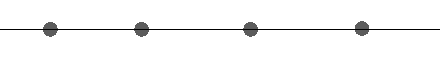
\includegraphics[width=\unitlength,page=1]{clipZ1.pdf}}%
    \put(0.1015445,0.01185338){\color[rgb]{0,0,0}\makebox(0,0)[b]{\smash{}}}%
    \put(0.0787076,0.00916782){\color[rgb]{0,0,0}\makebox(0,0)[lb]{\smash{$P₀$}}}%
    \put(0.79080231,0.01263303){\color[rgb]{0,0,0}\makebox(0,0)[lb]{\smash{$P₁$}}}%
    \put(0.076975,0.10619286){\color[rgb]{0,0,0}\makebox(0,0)[lb]{\smash{$t = 0$}}}%
    \put(0.76323075,0.1079256){\color[rgb]{0,0,0}\makebox(0,0)[lb]{\smash{$t = 1$}}}%
  \end{picture}%
\endgroup%


  setze $P₀ = P₀ + t₁ ΔP$, $P₁ = P₀ + t₂ ΔP$ mit $ΔP = P₁ - P₀$
\item $t₁, t₂ ∉ [0; 1]$
  \begin{enumerate}
  \item %% Creator: Inkscape inkscape 0.91, www.inkscape.org
%% PDF/EPS/PS + LaTeX output extension by Johan Engelen, 2010
%% Accompanies image file 'clipZ2.pdf' (pdf, eps, ps)
%%
%% To include the image in your LaTeX document, write
%%   \input{<filename>.pdf_tex}
%%  instead of
%%   \includegraphics{<filename>.pdf}
%% To scale the image, write
%%   \def\svgwidth{<desired width>}
%%   \input{<filename>.pdf_tex}
%%  instead of
%%   \includegraphics[width=<desired width>]{<filename>.pdf}
%%
%% Images with a different path to the parent latex file can
%% be accessed with the `import' package (which may need to be
%% installed) using
%%   \usepackage{import}
%% in the preamble, and then including the image with
%%   \import{<path to file>}{<filename>.pdf_tex}
%% Alternatively, one can specify
%%   \graphicspath{{<path to file>/}}
%% 
%% For more information, please see info/svg-inkscape on CTAN:
%%   http://tug.ctan.org/tex-archive/info/svg-inkscape
%%
\begingroup%
  \makeatletter%
  \providecommand\color[2][]{%
    \errmessage{(Inkscape) Color is used for the text in Inkscape, but the package 'color.sty' is not loaded}%
    \renewcommand\color[2][]{}%
  }%
  \providecommand\transparent[1]{%
    \errmessage{(Inkscape) Transparency is used (non-zero) for the text in Inkscape, but the package 'transparent.sty' is not loaded}%
    \renewcommand\transparent[1]{}%
  }%
  \providecommand\rotatebox[2]{#2}%
  \ifx\svgwidth\undefined%
    \setlength{\unitlength}{211.30308353bp}%
    \ifx\svgscale\undefined%
      \relax%
    \else%
      \setlength{\unitlength}{\unitlength * \real{\svgscale}}%
    \fi%
  \else%
    \setlength{\unitlength}{\svgwidth}%
  \fi%
  \global\let\svgwidth\undefined%
  \global\let\svgscale\undefined%
  \makeatother%
  \begin{picture}(1,0.08340291)%
    \put(0.08827299,0.00503387){\color[rgb]{0,0,0}\makebox(0,0)[lb]{\smash{$t₁$}}}%
    \put(0.79071078,0.00739853){\color[rgb]{0,0,0}\makebox(0,0)[lb]{\smash{$t₂$}}}%
    \put(0,0){
\includegraphics[width=\unitlength,page=1]{clipZ2.pdf}}%
    \put(0.1015445,0.01096873){\color[rgb]{0,0,0}\makebox(0,0)[b]{\smash{}}}%
    \put(0.29181623,0.00481783){\color[rgb]{0,0,0}\makebox(0,0)[lb]{\smash{$P₀$}}}%
    \put(0.5343789,0.00308537){\color[rgb]{0,0,0}\makebox(0,0)[lb]{\smash{$P₁$}}}%
  \end{picture}%
\endgroup%
 nichts zu tun
  \item %% Creator: Inkscape inkscape 0.91, www.inkscape.org
%% PDF/EPS/PS + LaTeX output extension by Johan Engelen, 2010
%% Accompanies image file 'clipZ3.pdf' (pdf, eps, ps)
%%
%% To include the image in your LaTeX document, write
%%   \input{<filename>.pdf_tex}
%%  instead of
%%   \includegraphics{<filename>.pdf}
%% To scale the image, write
%%   \def\svgwidth{<desired width>}
%%   \input{<filename>.pdf_tex}
%%  instead of
%%   \includegraphics[width=<desired width>]{<filename>.pdf}
%%
%% Images with a different path to the parent latex file can
%% be accessed with the `import' package (which may need to be
%% installed) using
%%   \usepackage{import}
%% in the preamble, and then including the image with
%%   \import{<path to file>}{<filename>.pdf_tex}
%% Alternatively, one can specify
%%   \graphicspath{{<path to file>/}}
%% 
%% For more information, please see info/svg-inkscape on CTAN:
%%   http://tug.ctan.org/tex-archive/info/svg-inkscape
%%
\begingroup%
  \makeatletter%
  \providecommand\color[2][]{%
    \errmessage{(Inkscape) Color is used for the text in Inkscape, but the package 'color.sty' is not loaded}%
    \renewcommand\color[2][]{}%
  }%
  \providecommand\transparent[1]{%
    \errmessage{(Inkscape) Transparency is used (non-zero) for the text in Inkscape, but the package 'transparent.sty' is not loaded}%
    \renewcommand\transparent[1]{}%
  }%
  \providecommand\rotatebox[2]{#2}%
  \ifx\svgwidth\undefined%
    \setlength{\unitlength}{211.30308353bp}%
    \ifx\svgscale\undefined%
      \relax%
    \else%
      \setlength{\unitlength}{\unitlength * \real{\svgscale}}%
    \fi%
  \else%
    \setlength{\unitlength}{\svgwidth}%
  \fi%
  \global\let\svgwidth\undefined%
  \global\let\svgscale\undefined%
  \makeatother%
  \begin{picture}(1,0.0814544)%
    \put(0.08827299,0.00308537){\color[rgb]{0,0,0}\makebox(0,0)[lb]{\smash{$t₁$}}}%
    \put(0.2917247,0.00718262){\color[rgb]{0,0,0}\makebox(0,0)[lb]{\smash{$t₂$}}}%
    \put(0,0){
\includegraphics[width=\unitlength,page=1]{clipZ3.pdf}}%
    \put(0.1015445,0.00902022){\color[rgb]{0,0,0}\makebox(0,0)[b]{\smash{}}}%
    \put(0.53957664,0.00806713){\color[rgb]{0,0,0}\makebox(0,0)[lb]{\smash{$P₀$}}}%
    \put(0.79080231,0.00979987){\color[rgb]{0,0,0}\makebox(0,0)[lb]{\smash{$P₁$}}}%
  \end{picture}%
\endgroup%
 zurückweisen
  \item %% Creator: Inkscape inkscape 0.91, www.inkscape.org
%% PDF/EPS/PS + LaTeX output extension by Johan Engelen, 2010
%% Accompanies image file 'clipZ4.pdf' (pdf, eps, ps)
%%
%% To include the image in your LaTeX document, write
%%   \input{<filename>.pdf_tex}
%%  instead of
%%   \includegraphics{<filename>.pdf}
%% To scale the image, write
%%   \def\svgwidth{<desired width>}
%%   \input{<filename>.pdf_tex}
%%  instead of
%%   \includegraphics[width=<desired width>]{<filename>.pdf}
%%
%% Images with a different path to the parent latex file can
%% be accessed with the `import' package (which may need to be
%% installed) using
%%   \usepackage{import}
%% in the preamble, and then including the image with
%%   \import{<path to file>}{<filename>.pdf_tex}
%% Alternatively, one can specify
%%   \graphicspath{{<path to file>/}}
%% 
%% For more information, please see info/svg-inkscape on CTAN:
%%   http://tug.ctan.org/tex-archive/info/svg-inkscape
%%
\begingroup%
  \makeatletter%
  \providecommand\color[2][]{%
    \errmessage{(Inkscape) Color is used for the text in Inkscape, but the package 'color.sty' is not loaded}%
    \renewcommand\color[2][]{}%
  }%
  \providecommand\transparent[1]{%
    \errmessage{(Inkscape) Transparency is used (non-zero) for the text in Inkscape, but the package 'transparent.sty' is not loaded}%
    \renewcommand\transparent[1]{}%
  }%
  \providecommand\rotatebox[2]{#2}%
  \ifx\svgwidth\undefined%
    \setlength{\unitlength}{211.30308353bp}%
    \ifx\svgscale\undefined%
      \relax%
    \else%
      \setlength{\unitlength}{\unitlength * \real{\svgscale}}%
    \fi%
  \else%
    \setlength{\unitlength}{\svgwidth}%
  \fi%
  \global\let\svgwidth\undefined%
  \global\let\svgscale\undefined%
  \makeatother%
  \begin{picture}(1,0.08513551)%
    \put(0.54047915,0.00676648){\color[rgb]{0,0,0}\makebox(0,0)[lb]{\smash{$t₁$}}}%
    \put(0.79071078,0.00913113){\color[rgb]{0,0,0}\makebox(0,0)[lb]{\smash{$t₂$}}}%
    \put(0,0){
\includegraphics[width=\unitlength,page=1]{clipZ4.pdf}}%
    \put(0.1015445,0.01270133){\color[rgb]{0,0,0}\makebox(0,0)[b]{\smash{}}}%
    \put(0.08737054,0.00655043){\color[rgb]{0,0,0}\makebox(0,0)[lb]{\smash{$P₀$}}}%
    \put(0.29008363,0.00308537){\color[rgb]{0,0,0}\makebox(0,0)[lb]{\smash{$P₁$}}}%
  \end{picture}%
\endgroup%
 zurückweisen
  \end{enumerate}
\item $t₁ ∈ (0; 1)$, $t₂ ∉ [0; 1]$

  %% Creator: Inkscape inkscape 0.91, www.inkscape.org
%% PDF/EPS/PS + LaTeX output extension by Johan Engelen, 2010
%% Accompanies image file 'clipZ5.pdf' (pdf, eps, ps)
%%
%% To include the image in your LaTeX document, write
%%   \input{<filename>.pdf_tex}
%%  instead of
%%   \includegraphics{<filename>.pdf}
%% To scale the image, write
%%   \def\svgwidth{<desired width>}
%%   \input{<filename>.pdf_tex}
%%  instead of
%%   \includegraphics[width=<desired width>]{<filename>.pdf}
%%
%% Images with a different path to the parent latex file can
%% be accessed with the `import' package (which may need to be
%% installed) using
%%   \usepackage{import}
%% in the preamble, and then including the image with
%%   \import{<path to file>}{<filename>.pdf_tex}
%% Alternatively, one can specify
%%   \graphicspath{{<path to file>/}}
%% 
%% For more information, please see info/svg-inkscape on CTAN:
%%   http://tug.ctan.org/tex-archive/info/svg-inkscape
%%
\begingroup%
  \makeatletter%
  \providecommand\color[2][]{%
    \errmessage{(Inkscape) Color is used for the text in Inkscape, but the package 'color.sty' is not loaded}%
    \renewcommand\color[2][]{}%
  }%
  \providecommand\transparent[1]{%
    \errmessage{(Inkscape) Transparency is used (non-zero) for the text in Inkscape, but the package 'transparent.sty' is not loaded}%
    \renewcommand\transparent[1]{}%
  }%
  \providecommand\rotatebox[2]{#2}%
  \ifx\svgwidth\undefined%
    \setlength{\unitlength}{211.30308353bp}%
    \ifx\svgscale\undefined%
      \relax%
    \else%
      \setlength{\unitlength}{\unitlength * \real{\svgscale}}%
    \fi%
  \else%
    \setlength{\unitlength}{\svgwidth}%
  \fi%
  \global\let\svgwidth\undefined%
  \global\let\svgscale\undefined%
  \makeatother%
  \begin{picture}(1,0.08167044)%
    \put(0.28752094,0.00503401){\color[rgb]{0,0,0}\makebox(0,0)[lb]{\smash{$t₁$}}}%
    \put(0.79071078,0.00566606){\color[rgb]{0,0,0}\makebox(0,0)[lb]{\smash{$t₂$}}}%
    \put(0,0){
\includegraphics[width=\unitlength,page=1]{clipZ5.pdf}}%
    \put(0.1015445,0.00923626){\color[rgb]{0,0,0}\makebox(0,0)[b]{\smash{}}}%
    \put(0.08737054,0.00308537){\color[rgb]{0,0,0}\makebox(0,0)[lb]{\smash{$P₀$}}}%
    \put(0.52918109,0.00655071){\color[rgb]{0,0,0}\makebox(0,0)[lb]{\smash{$P₁$}}}%
  \end{picture}%
\endgroup%
 $P₀ = P₀ + t₁ ΔP$
\item $t₁ ∉ [0; 1]$, $t₂ ∈ (0; 1)$

  %% Creator: Inkscape inkscape 0.91, www.inkscape.org
%% PDF/EPS/PS + LaTeX output extension by Johan Engelen, 2010
%% Accompanies image file 'clipZ6.pdf' (pdf, eps, ps)
%%
%% To include the image in your LaTeX document, write
%%   \input{<filename>.pdf_tex}
%%  instead of
%%   \includegraphics{<filename>.pdf}
%% To scale the image, write
%%   \def\svgwidth{<desired width>}
%%   \input{<filename>.pdf_tex}
%%  instead of
%%   \includegraphics[width=<desired width>]{<filename>.pdf}
%%
%% Images with a different path to the parent latex file can
%% be accessed with the `import' package (which may need to be
%% installed) using
%%   \usepackage{import}
%% in the preamble, and then including the image with
%%   \import{<path to file>}{<filename>.pdf_tex}
%% Alternatively, one can specify
%%   \graphicspath{{<path to file>/}}
%% 
%% For more information, please see info/svg-inkscape on CTAN:
%%   http://tug.ctan.org/tex-archive/info/svg-inkscape
%%
\begingroup%
  \makeatletter%
  \providecommand\color[2][]{%
    \errmessage{(Inkscape) Color is used for the text in Inkscape, but the package 'color.sty' is not loaded}%
    \renewcommand\color[2][]{}%
  }%
  \providecommand\transparent[1]{%
    \errmessage{(Inkscape) Transparency is used (non-zero) for the text in Inkscape, but the package 'transparent.sty' is not loaded}%
    \renewcommand\transparent[1]{}%
  }%
  \providecommand\rotatebox[2]{#2}%
  \ifx\svgwidth\undefined%
    \setlength{\unitlength}{211.30308353bp}%
    \ifx\svgscale\undefined%
      \relax%
    \else%
      \setlength{\unitlength}{\unitlength * \real{\svgscale}}%
    \fi%
  \else%
    \setlength{\unitlength}{\svgwidth}%
  \fi%
  \global\let\svgwidth\undefined%
  \global\let\svgscale\undefined%
  \makeatother%
  \begin{picture}(1,0.0797218)%
    \put(0.09173819,0.00308537){\color[rgb]{0,0,0}\makebox(0,0)[lb]{\smash{$t₁$}}}%
    \put(0.54295031,0.00718262){\color[rgb]{0,0,0}\makebox(0,0)[lb]{\smash{$t₂$}}}%
    \put(0,0){
\includegraphics[width=\unitlength,page=1]{clipZ6.pdf}}%
    \put(0.1015445,0.00728762){\color[rgb]{0,0,0}\makebox(0,0)[b]{\smash{}}}%
    \put(0.28488589,0.0097996){\color[rgb]{0,0,0}\makebox(0,0)[lb]{\smash{$P₀$}}}%
    \put(0.79080218,0.00633467){\color[rgb]{0,0,0}\makebox(0,0)[lb]{\smash{$P₁$}}}%
  \end{picture}%
\endgroup%
 $P₁ = P₁ + t₂ ΔP$
\end{enumerate}

\minisec{Clipping für Fall~\ref{it:clipx}}

\begin{enumerate}
\item $z(t₁) > 0$, $z(t₂) > 0$

  %% Creator: Inkscape inkscape 0.91, www.inkscape.org
%% PDF/EPS/PS + LaTeX output extension by Johan Engelen, 2010
%% Accompanies image file 'clipX1.pdf' (pdf, eps, ps)
%%
%% To include the image in your LaTeX document, write
%%   \input{<filename>.pdf_tex}
%%  instead of
%%   \includegraphics{<filename>.pdf}
%% To scale the image, write
%%   \def\svgwidth{<desired width>}
%%   \input{<filename>.pdf_tex}
%%  instead of
%%   \includegraphics[width=<desired width>]{<filename>.pdf}
%%
%% Images with a different path to the parent latex file can
%% be accessed with the `import' package (which may need to be
%% installed) using
%%   \usepackage{import}
%% in the preamble, and then including the image with
%%   \import{<path to file>}{<filename>.pdf_tex}
%% Alternatively, one can specify
%%   \graphicspath{{<path to file>/}}
%% 
%% For more information, please see info/svg-inkscape on CTAN:
%%   http://tug.ctan.org/tex-archive/info/svg-inkscape
%%
\begingroup%
  \makeatletter%
  \providecommand\color[2][]{%
    \errmessage{(Inkscape) Color is used for the text in Inkscape, but the package 'color.sty' is not loaded}%
    \renewcommand\color[2][]{}%
  }%
  \providecommand\transparent[1]{%
    \errmessage{(Inkscape) Transparency is used (non-zero) for the text in Inkscape, but the package 'transparent.sty' is not loaded}%
    \renewcommand\transparent[1]{}%
  }%
  \providecommand\rotatebox[2]{#2}%
  \ifx\svgwidth\undefined%
    \setlength{\unitlength}{148.23673966bp}%
    \ifx\svgscale\undefined%
      \relax%
    \else%
      \setlength{\unitlength}{\unitlength * \real{\svgscale}}%
    \fi%
  \else%
    \setlength{\unitlength}{\svgwidth}%
  \fi%
  \global\let\svgwidth\undefined%
  \global\let\svgscale\undefined%
  \makeatother%
  \begin{picture}(1,0.95779575)%
    \put(0.36783106,0.56908493){\color[rgb]{0,0,0}\makebox(0,0)[lb]{\smash{$t₁$}}}%
    \put(0.50603544,0.59064523){\color[rgb]{0,0,0}\makebox(0,0)[lb]{\smash{$t₂$}}}%
    \put(0,0){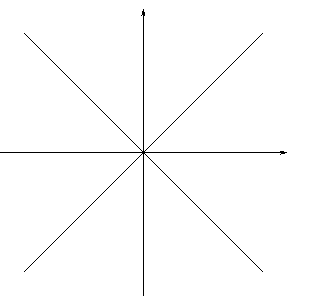
\includegraphics[width=\unitlength,page=1]{clipX1.pdf}}%
    \put(0.48743511,0.92836984){\color[rgb]{0,0,0}\makebox(0,0)[lb]{\smash{$z$}}}%
    \put(0.93606532,0.47973959){\color[rgb]{0,0,0}\makebox(0,0)[lb]{\smash{$x$}}}%
    \put(0.86647857,0.0697505){\color[rgb]{0,0,0}\makebox(0,0)[lb]{\smash{$z = -x$}}}%
    \put(0.85861931,0.84322834){\color[rgb]{0,0,0}\makebox(0,0)[lb]{\smash{$z = x$}}}%
    \put(0,0){\includegraphics[width=\unitlength,page=2]{clipX1.pdf}}%
  \end{picture}%
\endgroup%
 \qquad ⇒ zurückweisen
\item $z(t₁) ≤ 0$, $z(t₂) ≤ 0$

  %% Creator: Inkscape inkscape 0.91, www.inkscape.org
%% PDF/EPS/PS + LaTeX output extension by Johan Engelen, 2010
%% Accompanies image file 'clipX2.pdf' (pdf, eps, ps)
%%
%% To include the image in your LaTeX document, write
%%   \input{<filename>.pdf_tex}
%%  instead of
%%   \includegraphics{<filename>.pdf}
%% To scale the image, write
%%   \def\svgwidth{<desired width>}
%%   \input{<filename>.pdf_tex}
%%  instead of
%%   \includegraphics[width=<desired width>]{<filename>.pdf}
%%
%% Images with a different path to the parent latex file can
%% be accessed with the `import' package (which may need to be
%% installed) using
%%   \usepackage{import}
%% in the preamble, and then including the image with
%%   \import{<path to file>}{<filename>.pdf_tex}
%% Alternatively, one can specify
%%   \graphicspath{{<path to file>/}}
%% 
%% For more information, please see info/svg-inkscape on CTAN:
%%   http://tug.ctan.org/tex-archive/info/svg-inkscape
%%
\begingroup%
  \makeatletter%
  \providecommand\color[2][]{%
    \errmessage{(Inkscape) Color is used for the text in Inkscape, but the package 'color.sty' is not loaded}%
    \renewcommand\color[2][]{}%
  }%
  \providecommand\transparent[1]{%
    \errmessage{(Inkscape) Transparency is used (non-zero) for the text in Inkscape, but the package 'transparent.sty' is not loaded}%
    \renewcommand\transparent[1]{}%
  }%
  \providecommand\rotatebox[2]{#2}%
  \ifx\svgwidth\undefined%
    \setlength{\unitlength}{147.50127155bp}%
    \ifx\svgscale\undefined%
      \relax%
    \else%
      \setlength{\unitlength}{\unitlength * \real{\svgscale}}%
    \fi%
  \else%
    \setlength{\unitlength}{\svgwidth}%
  \fi%
  \global\let\svgwidth\undefined%
  \global\let\svgscale\undefined%
  \makeatother%
  \begin{picture}(1,0.96257149)%
    \put(0.29768644,0.2529824){\color[rgb]{0,0,0}\makebox(0,0)[lb]{\smash{$t₁$}}}%
    \put(0.54702997,0.28333725){\color[rgb]{0,0,0}\makebox(0,0)[lb]{\smash{$t₂$}}}%
    \put(0,0){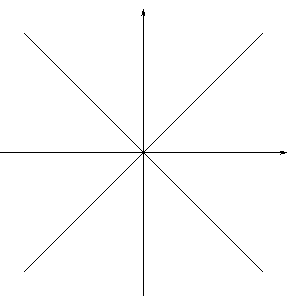
\includegraphics[width=\unitlength,page=1]{clipX2.pdf}}%
    \put(0.48986555,0.93299887){\color[rgb]{0,0,0}\makebox(0,0)[lb]{\smash{$z$}}}%
    \put(0.94073271,0.48213166){\color[rgb]{0,0,0}\makebox(0,0)[lb]{\smash{$x$}}}%
    \put(0,0){\includegraphics[width=\unitlength,page=2]{clipX2.pdf}}%
  \end{picture}%
\endgroup%
 \qquad ⇒ Standard-Clipping wie im Fall~\ref{it:clipz}
  
  \pagebreak

\item Annahme: $z₀ < z₁$, sonst vertausche $P₀$ und $P₁$

  $tᵤ := \min\{t₁, t₂\}$ (unterer Schnittpunkt), $tₒ := \max\{t₁, t₂\}$ (oberer Schnittpunkt)

  damit hier $z(tᵤ) ≤ 0$, $z(tₒ) > 0$
  \begin{enumerate}
  \item $tᵤ < 0$:

    %% Creator: Inkscape inkscape 0.91, www.inkscape.org
%% PDF/EPS/PS + LaTeX output extension by Johan Engelen, 2010
%% Accompanies image file 'clipX3.pdf' (pdf, eps, ps)
%%
%% To include the image in your LaTeX document, write
%%   \input{<filename>.pdf_tex}
%%  instead of
%%   \includegraphics{<filename>.pdf}
%% To scale the image, write
%%   \def\svgwidth{<desired width>}
%%   \input{<filename>.pdf_tex}
%%  instead of
%%   \includegraphics[width=<desired width>]{<filename>.pdf}
%%
%% Images with a different path to the parent latex file can
%% be accessed with the `import' package (which may need to be
%% installed) using
%%   \usepackage{import}
%% in the preamble, and then including the image with
%%   \import{<path to file>}{<filename>.pdf_tex}
%% Alternatively, one can specify
%%   \graphicspath{{<path to file>/}}
%% 
%% For more information, please see info/svg-inkscape on CTAN:
%%   http://tug.ctan.org/tex-archive/info/svg-inkscape
%%
\begingroup%
  \makeatletter%
  \providecommand\color[2][]{%
    \errmessage{(Inkscape) Color is used for the text in Inkscape, but the package 'color.sty' is not loaded}%
    \renewcommand\color[2][]{}%
  }%
  \providecommand\transparent[1]{%
    \errmessage{(Inkscape) Transparency is used (non-zero) for the text in Inkscape, but the package 'transparent.sty' is not loaded}%
    \renewcommand\transparent[1]{}%
  }%
  \providecommand\rotatebox[2]{#2}%
  \ifx\svgwidth\undefined%
    \setlength{\unitlength}{138.52657314bp}%
    \ifx\svgscale\undefined%
      \relax%
    \else%
      \setlength{\unitlength}{\unitlength * \real{\svgscale}}%
    \fi%
  \else%
    \setlength{\unitlength}{\svgwidth}%
  \fi%
  \global\let\svgwidth\undefined%
  \global\let\svgscale\undefined%
  \makeatother%
  \begin{picture}(1,1.00017521)%
    \put(0.29715137,0.24690825){\color[rgb]{0,0,0}\makebox(0,0)[lb]{\smash{$tᵤ$}}}%
    \put(0.40143672,0.59108325){\color[rgb]{0,0,0}\makebox(0,0)[lb]{\smash{$tₒ$}}}%
    \put(0,0){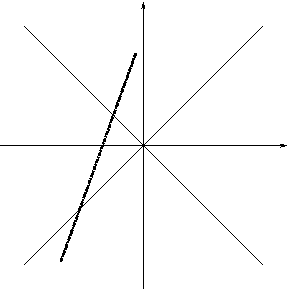
\includegraphics[width=\unitlength,page=1]{clipX3.pdf}}%
    \put(0.13493916,0.53452634){\color[rgb]{0,0,0}\makebox(0,0)[lb]{\smash{$P₀$}}}%
    \put(0.15608182,0.6045613){\color[rgb]{0,0,0}\makebox(0,0)[lb]{\smash{$P₁$}}}%
    \put(0,0){\includegraphics[width=\unitlength,page=2]{clipX3.pdf}}%
  \end{picture}%
\endgroup%
 \qquad ⇒ zurückweisen
  \item $tᵤ ≥ 1$:

    %% Creator: Inkscape inkscape 0.91, www.inkscape.org
%% PDF/EPS/PS + LaTeX output extension by Johan Engelen, 2010
%% Accompanies image file 'clipX4.pdf' (pdf, eps, ps)
%%
%% To include the image in your LaTeX document, write
%%   \input{<filename>.pdf_tex}
%%  instead of
%%   \includegraphics{<filename>.pdf}
%% To scale the image, write
%%   \def\svgwidth{<desired width>}
%%   \input{<filename>.pdf_tex}
%%  instead of
%%   \includegraphics[width=<desired width>]{<filename>.pdf}
%%
%% Images with a different path to the parent latex file can
%% be accessed with the `import' package (which may need to be
%% installed) using
%%   \usepackage{import}
%% in the preamble, and then including the image with
%%   \import{<path to file>}{<filename>.pdf_tex}
%% Alternatively, one can specify
%%   \graphicspath{{<path to file>/}}
%% 
%% For more information, please see info/svg-inkscape on CTAN:
%%   http://tug.ctan.org/tex-archive/info/svg-inkscape
%%
\begingroup%
  \makeatletter%
  \providecommand\color[2][]{%
    \errmessage{(Inkscape) Color is used for the text in Inkscape, but the package 'color.sty' is not loaded}%
    \renewcommand\color[2][]{}%
  }%
  \providecommand\transparent[1]{%
    \errmessage{(Inkscape) Transparency is used (non-zero) for the text in Inkscape, but the package 'transparent.sty' is not loaded}%
    \renewcommand\transparent[1]{}%
  }%
  \providecommand\rotatebox[2]{#2}%
  \ifx\svgwidth\undefined%
    \setlength{\unitlength}{138.52657314bp}%
    \ifx\svgscale\undefined%
      \relax%
    \else%
      \setlength{\unitlength}{\unitlength * \real{\svgscale}}%
    \fi%
  \else%
    \setlength{\unitlength}{\svgwidth}%
  \fi%
  \global\let\svgwidth\undefined%
  \global\let\svgscale\undefined%
  \makeatother%
  \begin{picture}(1,1.00017521)%
    \put(0.29715137,0.24690825){\color[rgb]{0,0,0}\makebox(0,0)[lb]{\smash{$tᵤ$}}}%
    \put(0.40143672,0.59108325){\color[rgb]{0,0,0}\makebox(0,0)[lb]{\smash{$tₒ$}}}%
    \put(0,0){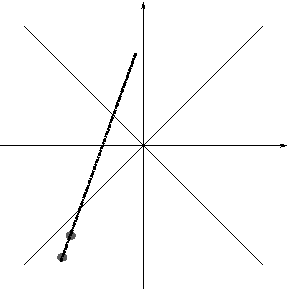
\includegraphics[width=\unitlength,page=1]{clipX4.pdf}}%
    \put(0.23536652,0.08656723){\color[rgb]{0,0,0}\makebox(0,0)[lb]{\smash{$P₀$}}}%
    \put(0.2644376,0.16585204){\color[rgb]{0,0,0}\makebox(0,0)[lb]{\smash{$P₁$}}}%
    \put(0,0){\includegraphics[width=\unitlength,page=2]{clipX4.pdf}}%
  \end{picture}%
\endgroup%
 \qquad ⇒ nichts zu tun (alles sichtbar)
  \item $0 ≤ tᵤ < 1$:

    %% Creator: Inkscape inkscape 0.91, www.inkscape.org
%% PDF/EPS/PS + LaTeX output extension by Johan Engelen, 2010
%% Accompanies image file 'clipX5.pdf' (pdf, eps, ps)
%%
%% To include the image in your LaTeX document, write
%%   \input{<filename>.pdf_tex}
%%  instead of
%%   \includegraphics{<filename>.pdf}
%% To scale the image, write
%%   \def\svgwidth{<desired width>}
%%   \input{<filename>.pdf_tex}
%%  instead of
%%   \includegraphics[width=<desired width>]{<filename>.pdf}
%%
%% Images with a different path to the parent latex file can
%% be accessed with the `import' package (which may need to be
%% installed) using
%%   \usepackage{import}
%% in the preamble, and then including the image with
%%   \import{<path to file>}{<filename>.pdf_tex}
%% Alternatively, one can specify
%%   \graphicspath{{<path to file>/}}
%% 
%% For more information, please see info/svg-inkscape on CTAN:
%%   http://tug.ctan.org/tex-archive/info/svg-inkscape
%%
\begingroup%
  \makeatletter%
  \providecommand\color[2][]{%
    \errmessage{(Inkscape) Color is used for the text in Inkscape, but the package 'color.sty' is not loaded}%
    \renewcommand\color[2][]{}%
  }%
  \providecommand\transparent[1]{%
    \errmessage{(Inkscape) Transparency is used (non-zero) for the text in Inkscape, but the package 'transparent.sty' is not loaded}%
    \renewcommand\transparent[1]{}%
  }%
  \providecommand\rotatebox[2]{#2}%
  \ifx\svgwidth\undefined%
    \setlength{\unitlength}{138.52657314bp}%
    \ifx\svgscale\undefined%
      \relax%
    \else%
      \setlength{\unitlength}{\unitlength * \real{\svgscale}}%
    \fi%
  \else%
    \setlength{\unitlength}{\svgwidth}%
  \fi%
  \global\let\svgwidth\undefined%
  \global\let\svgscale\undefined%
  \makeatother%
  \begin{picture}(1,1.00017521)%
    \put(0.29715137,0.24690825){\color[rgb]{0,0,0}\makebox(0,0)[lb]{\smash{$tᵤ$}}}%
    \put(0.40143672,0.59108325){\color[rgb]{0,0,0}\makebox(0,0)[lb]{\smash{$tₒ$}}}%
    \put(0,0){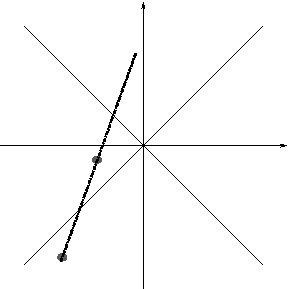
\includegraphics[width=\unitlength,page=1]{clipX5.pdf}}%
    \put(0.23536652,0.08656723){\color[rgb]{0,0,0}\makebox(0,0)[lb]{\smash{$P₀$}}}%
    \put(0.21025971,0.4169206){\color[rgb]{0,0,0}\makebox(0,0)[lb]{\smash{$P₁$}}}%
    \put(0,0){\includegraphics[width=\unitlength,page=2]{clipX5.pdf}}%
  \end{picture}%
\endgroup%
 \qquad ⇒ $P₁ = P₁ + tᵤ ΔP$
  \end{enumerate}
\end{enumerate}

\end{document}
